\chapter{Curve Rendering}

As a sketching application, it is important for curves to be rendered with high quality.
While graphics hardware has support for line rendering, it's implementation is only suitable for line segments, with significant issues when trying to render curves.
In this chapter, we discuss a new system which we implemented for curve rendering.

\section{Problems with Native Curve Renderering}
OpenGL has support for a variety of line primitives: lines, line strips, and lines with adjacency data.
However, these primitives are not suited for rendering curves at high quality.
This is because OpenGL uses a rectangle between the two segment points to render line segments.
While this method is well-suited for common uses of lines in 3D applications, for example wire frame images, it does not extend to curve rendering because of the gaps that appear between segments (Figure~\ref{fig:gllineartifact}).
It is reasonable to assume that if we use a curve that is subdivided to a fine enough degree, then the gaps will be sufficiently small that they would not be visible.
However, in practice, in many cases even finely subdivided lines have visible gaps around any curve (Figure~\ref{fig:glexample}). 

\begin{figure}
\label{fig:gllineartifact}
	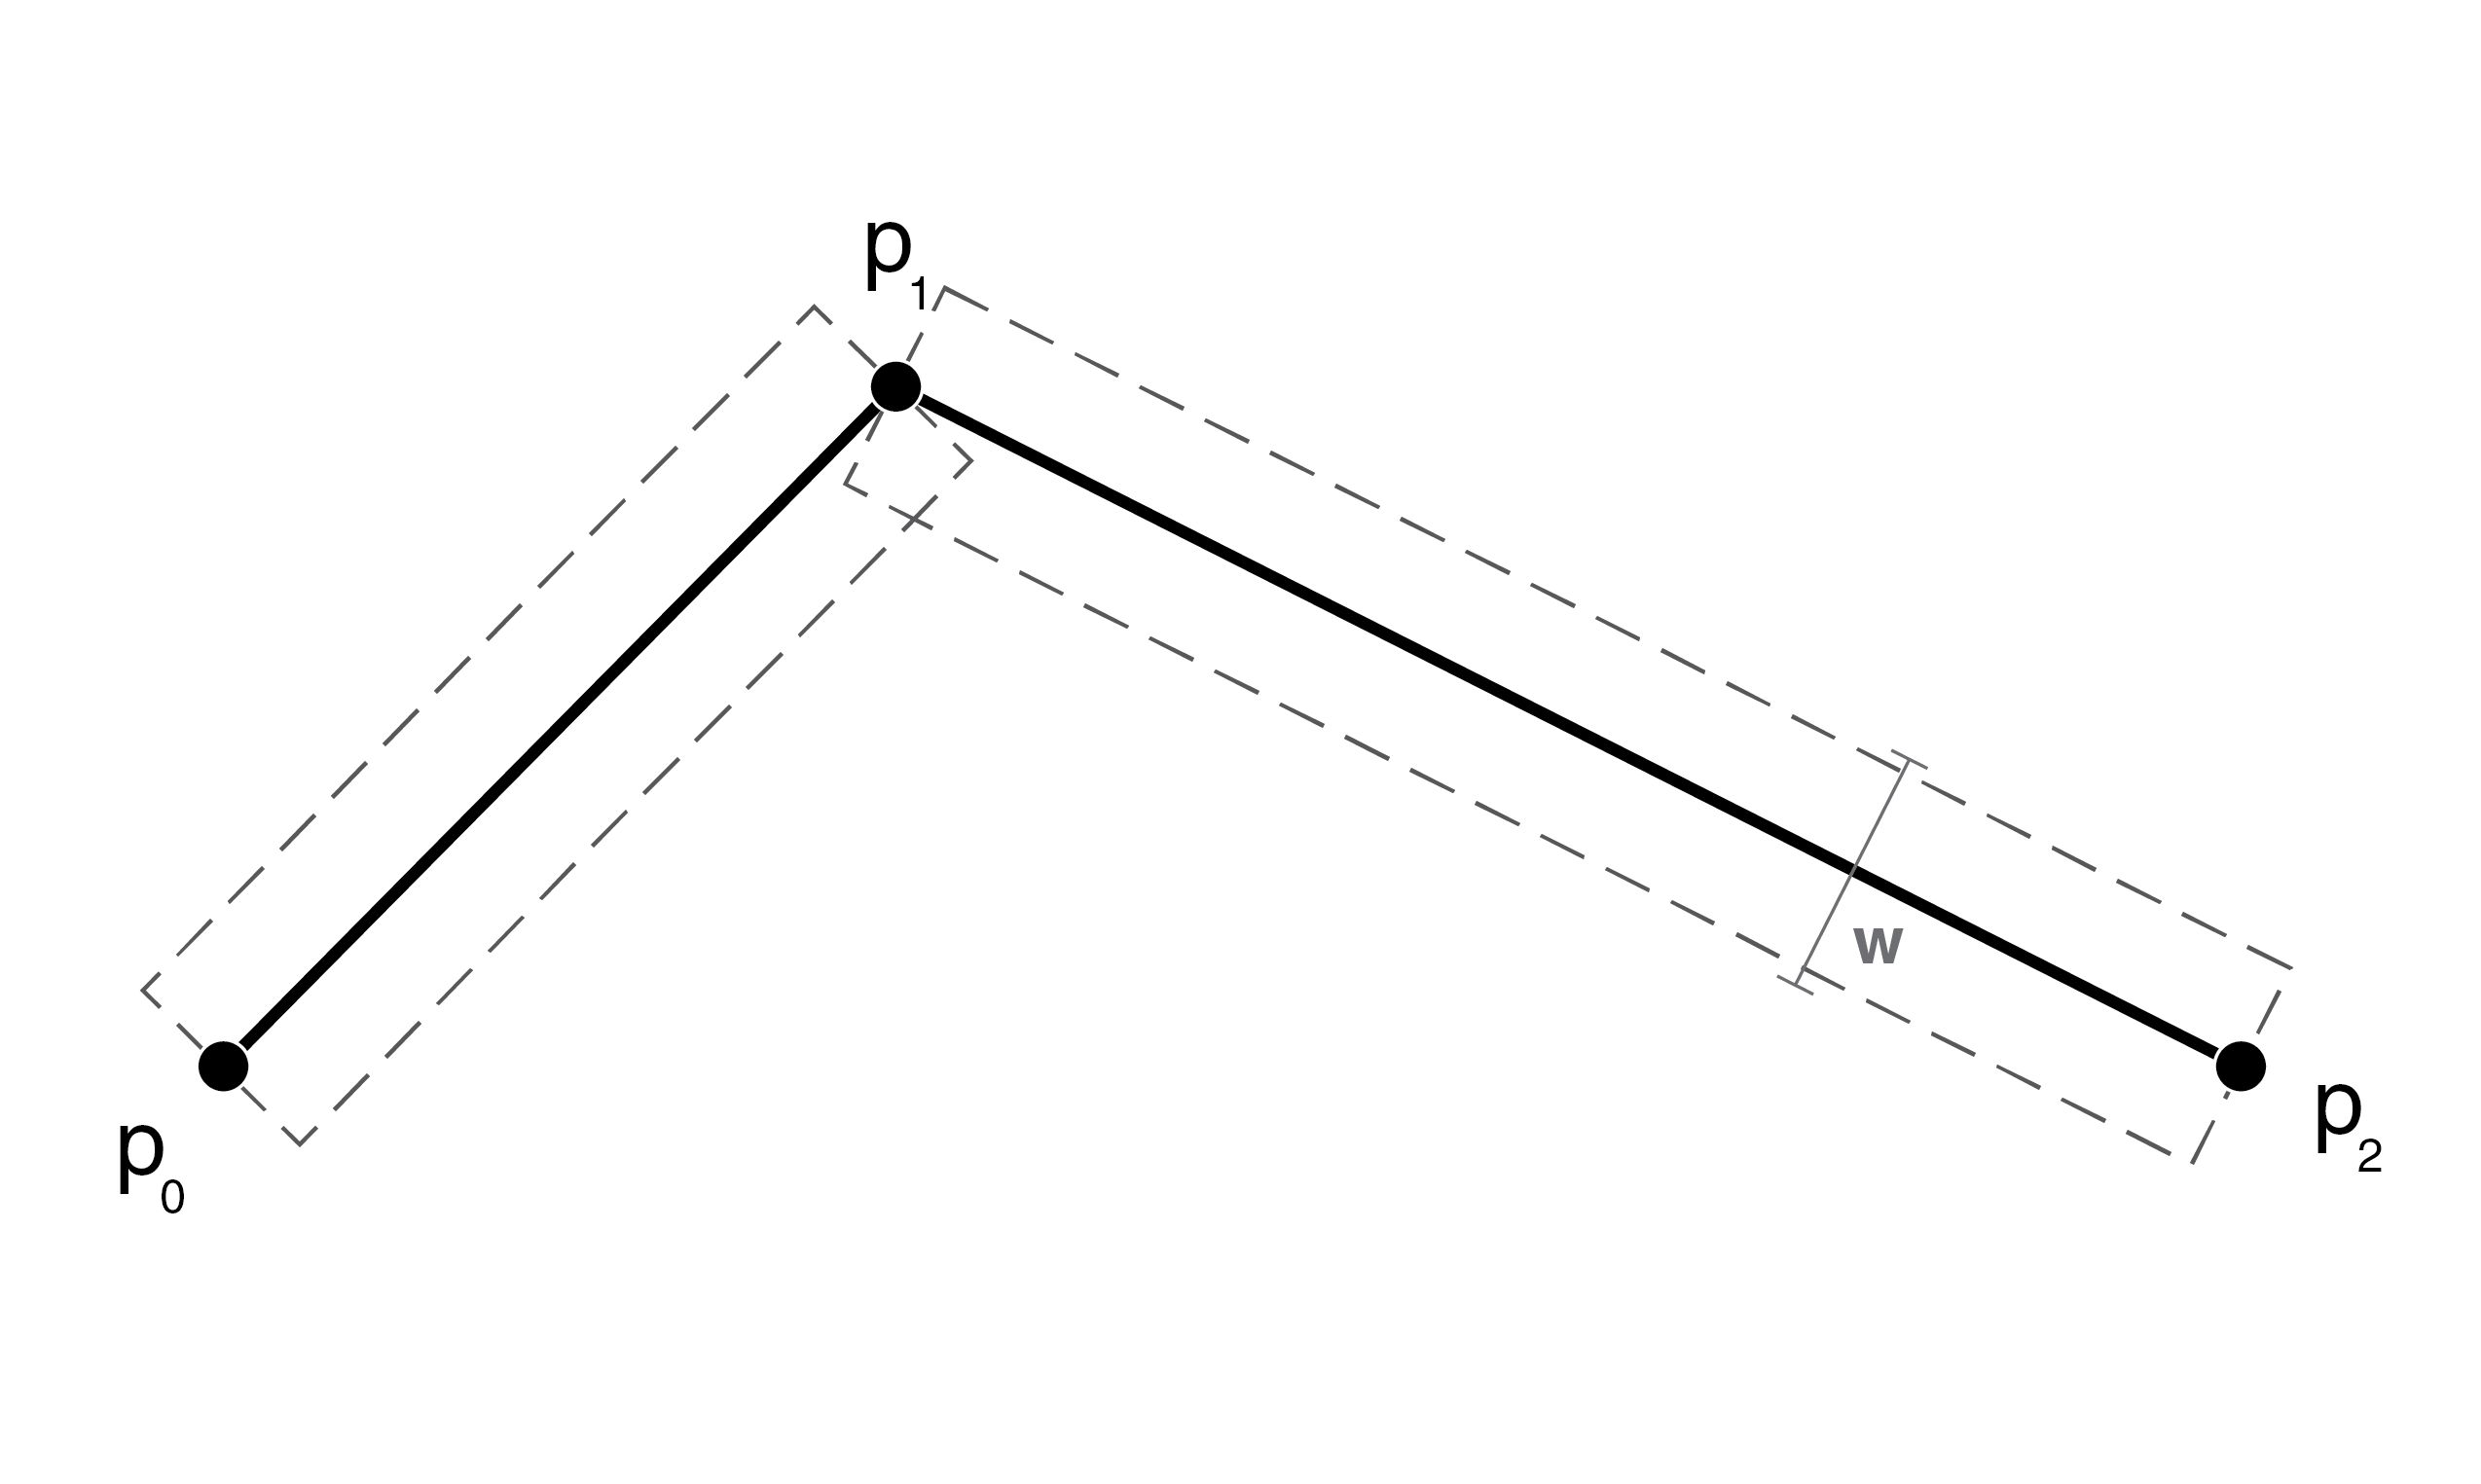
\includegraphics[width=\textwidth]{linesegment2.png}
	\caption[Artifacts with GL\_LINES]{Two line segments connected together, as displayed by the default GL\_LINES implementation. The dotted lines represent the geometry created from the line definitions. Note the visible artifact at their intersection.}
\end{figure}

To eliminate these artifacts, our project implements a custom line renderer that constructs a triangle mesh from the line definition.
Constructing a mesh for the line allow allows the implementation of a wide variety of stroke types, including strokes with various end caps or variable widths based on stroke direction. 
Additionally, OpenGL lines have inconsistent support for anti-aliasing across all hardware.
By switching to a triangle mesh, we leverage the native anti-aliasing support for triangles without worrying about consistency.
As we can see in the above image, without anti-aliasing rendered lines can appear jagged and of poor quality.
In order for our system to be visibly appealing in sketch mode, it is important to render the highest quality lines as possible.

\begin{figure}
\label{fig:glexample}
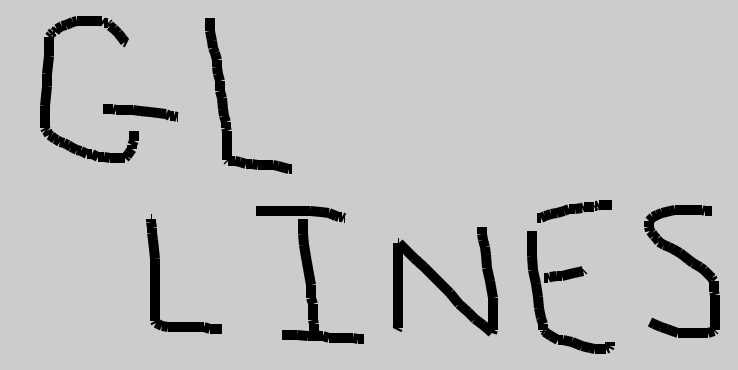
\includegraphics[width=\linewidth]{gllines}
\caption[Flaws in GL\_LINES]{An example of the flaws of using native line rendering in OpenGL with GL\_LINES for rendering our sketch data. The cause of the holes is the artifact in Figure~\ref{fig:gllineartifact}.}
\end{figure}

\section{Creating Joins From the Curve Definition}

\begin{table}
\begin{center}
\begin{tabular}{|c|l|}
\hline
\textbf{Symbol} & \textbf{Description} \\ \hline
$p_n$			& Ordered point on line in the range $[0,2]$ \\
$w$				& The width of the rectangular line segments \\
$\vec{n_{xy}}$		& The normal to the line segment $(p_x, p_y)$ \\	
$\vec{t_x}$			& Vector from $p_1$ along $n_{x1}$ with length $w/2$ \\
\hline
\end{tabular}
\caption{Section Variables} \label{tab:linevariables}
\end{center}
\end{table}

To improve the appearance of our curved lines relative to the native OpenGL implementation, it is necessary to compute better methods for rendering the intersections between each of our line segments.
For this project, we implement three types of "joins": round, miter, and bevel.
Miter and bevel joins are used in conjunction with each other, while round joins are used alone.

A round join (Figure~\ref{fig:roundjoin}) is formed by rounding out the gap such that a smooth curve is created. 
If both of our line segments have the same thickness, then the join calculated by forming a circle whose center is located at $p_1$, with a radius of $w/2$. 
The total angle that needs to be filled can be calculated by $\vec{t_0} \cdot \vec{t_2}$, and can be filled by rotating either $\vec{t_0}$ or $\vec{t_2}$ about $p_1$. 

Miter joins are formed by extending the lines in the line geometry parallel to the original segment.
The join is formed where these extended lines intersect, as can be seen in Figure~\ref{fig:miterjoin}.
To calculate this, we take the vectors defined by $(p_0 + \vec{t_0}, p_1 + \vec{t_0})$ and $(p_2 + \vec{t_2}, p_1 + \vec{t_2})$ and compute their intersection. We call the vector from $p_1$ to this intersection $\vec{v}$.
We can then compute a polygon between $p_1$, $p_1 + \vec{t_0}$, $p_1 + \vec{t_2}$, and $p_1 + \vec{v}$, which creates the miter join. 

\begin{figure}
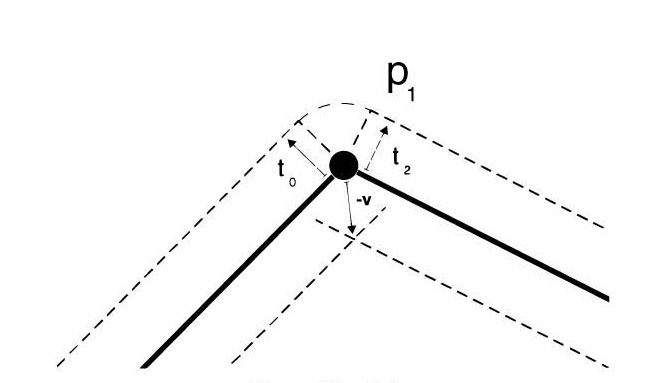
\includegraphics[width=0.7\textwidth]{round.jpg}
\caption[Round Join Diagram]{Diagram of a round join with parameter labels. The smooth curve is approximated with a triangularization.}
\label{fig:roundjoin}
\end{figure}

\begin{figure}
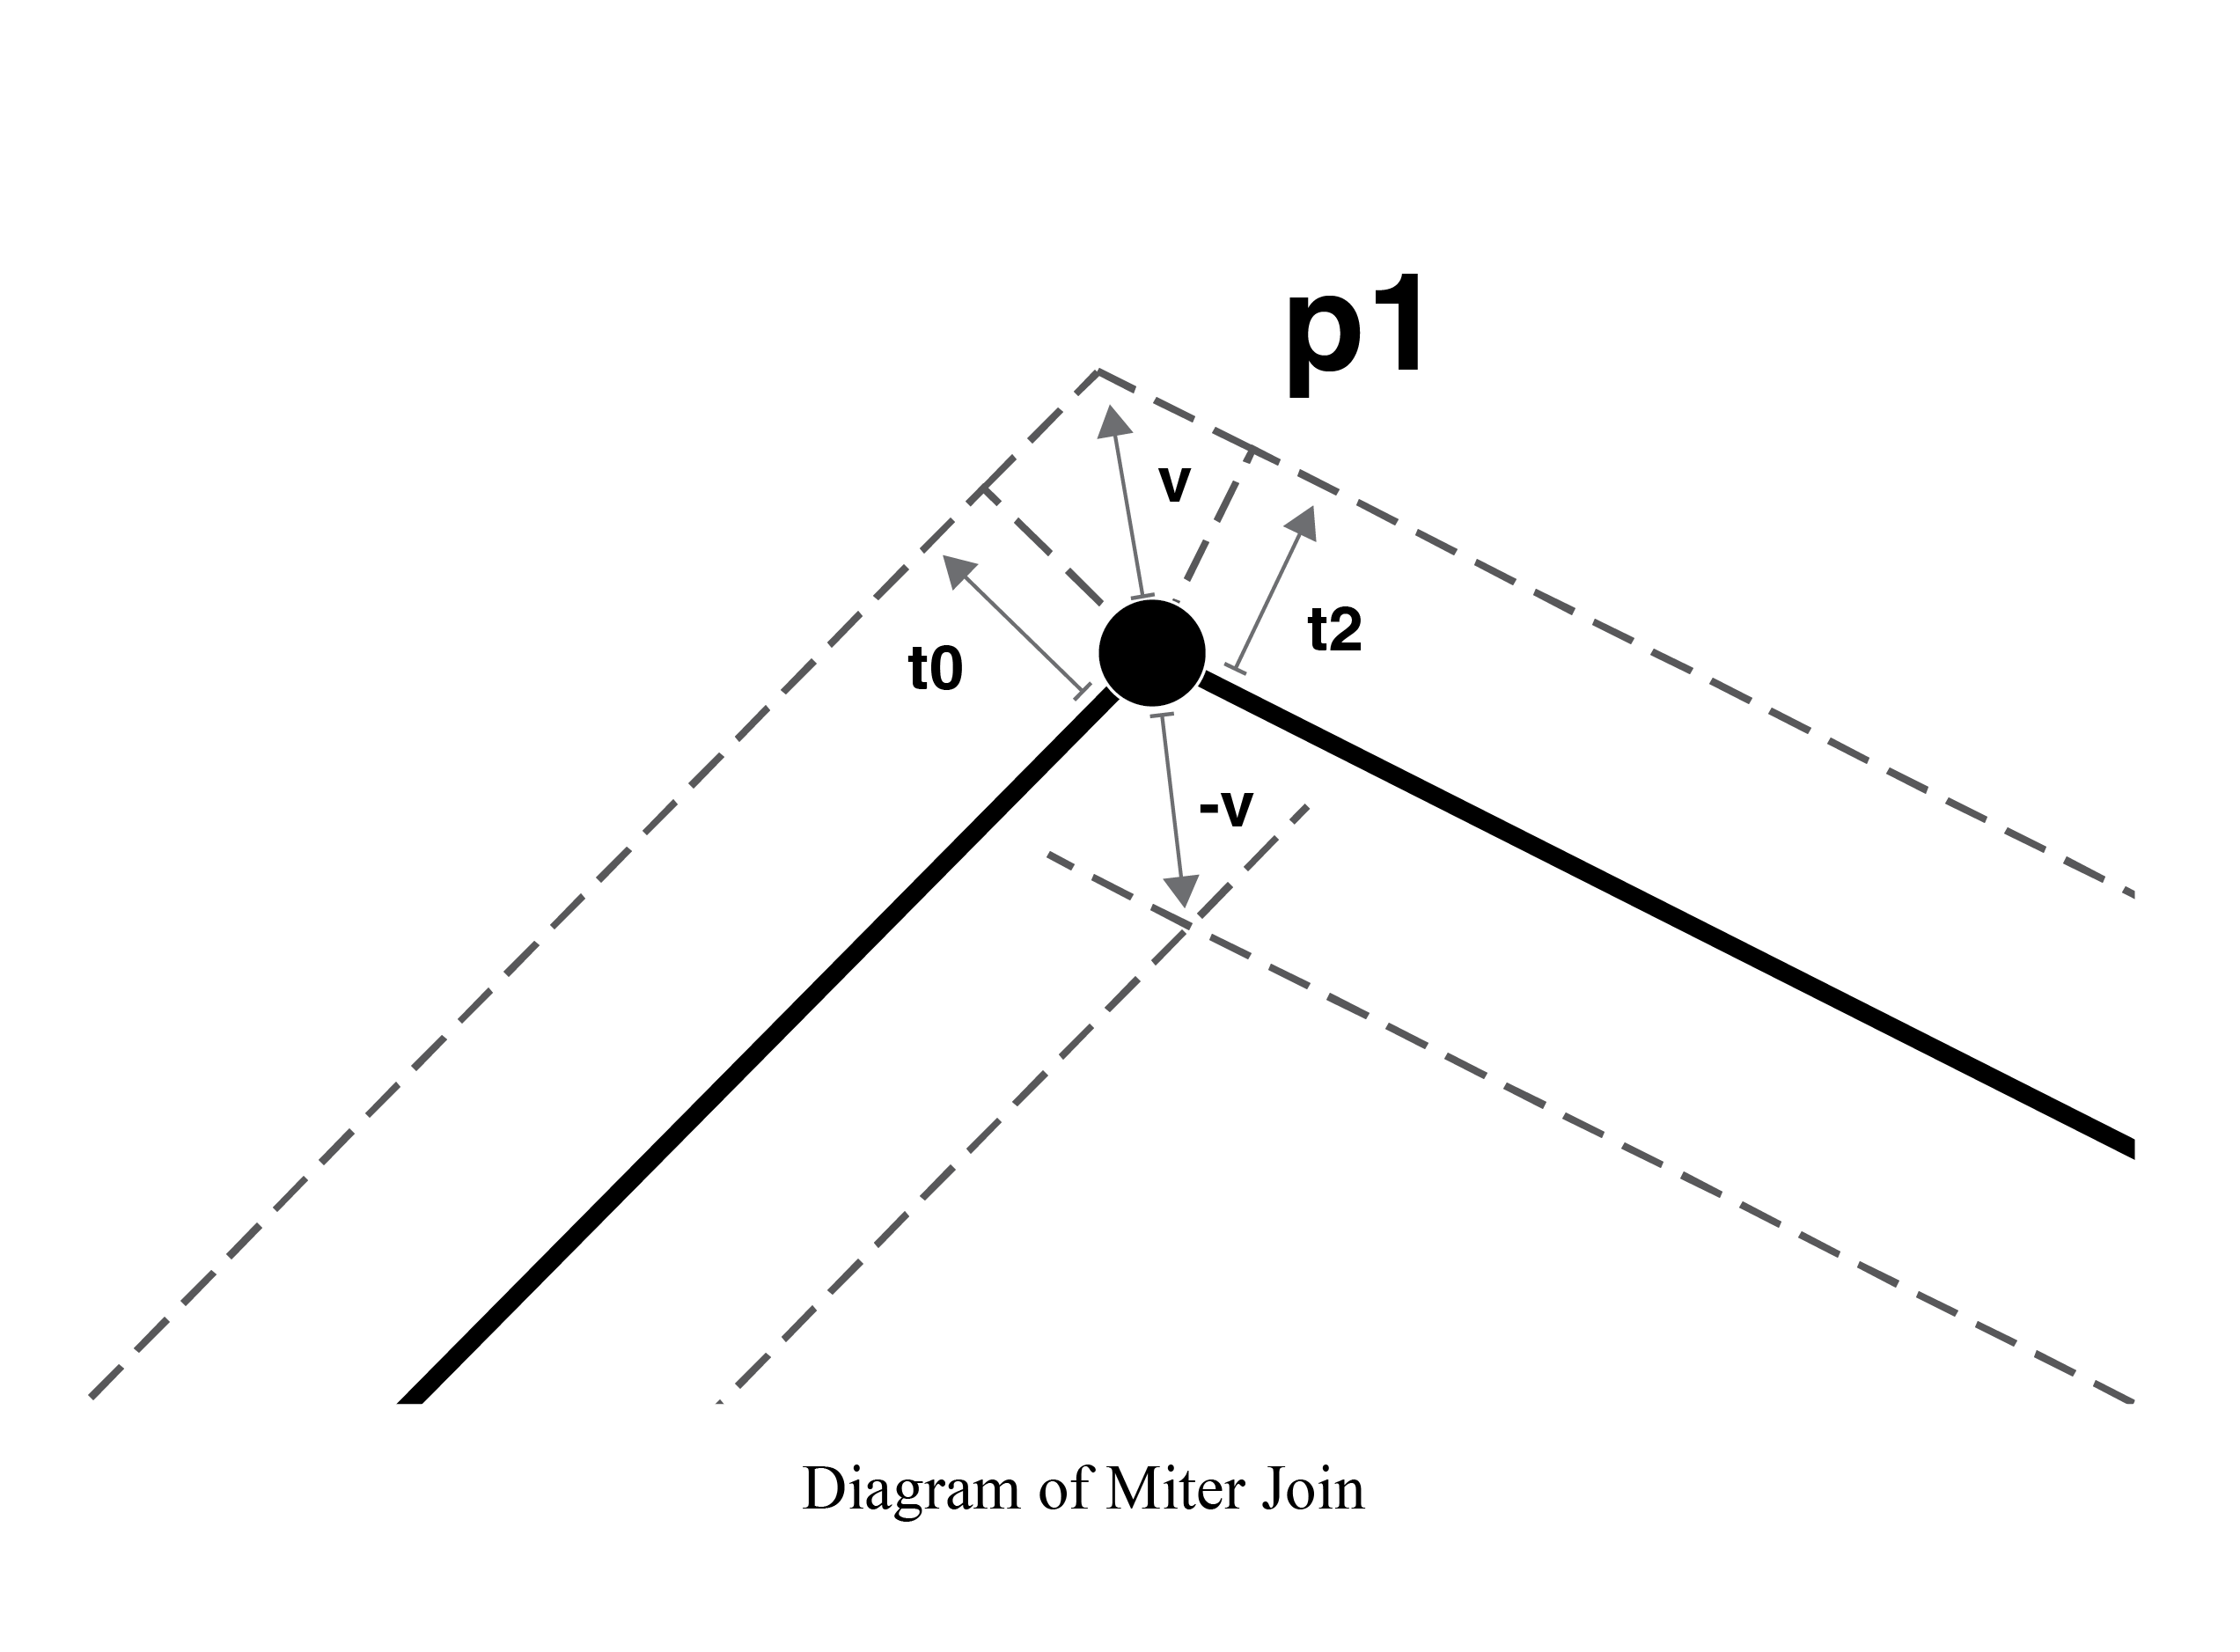
\includegraphics[width=0.7\textwidth]{miter.png}
\caption[Miter Join Diagram]{Diagram of a miter join with parameter labels}
\label{fig:miterjoin}
\end{figure}

\begin{figure}
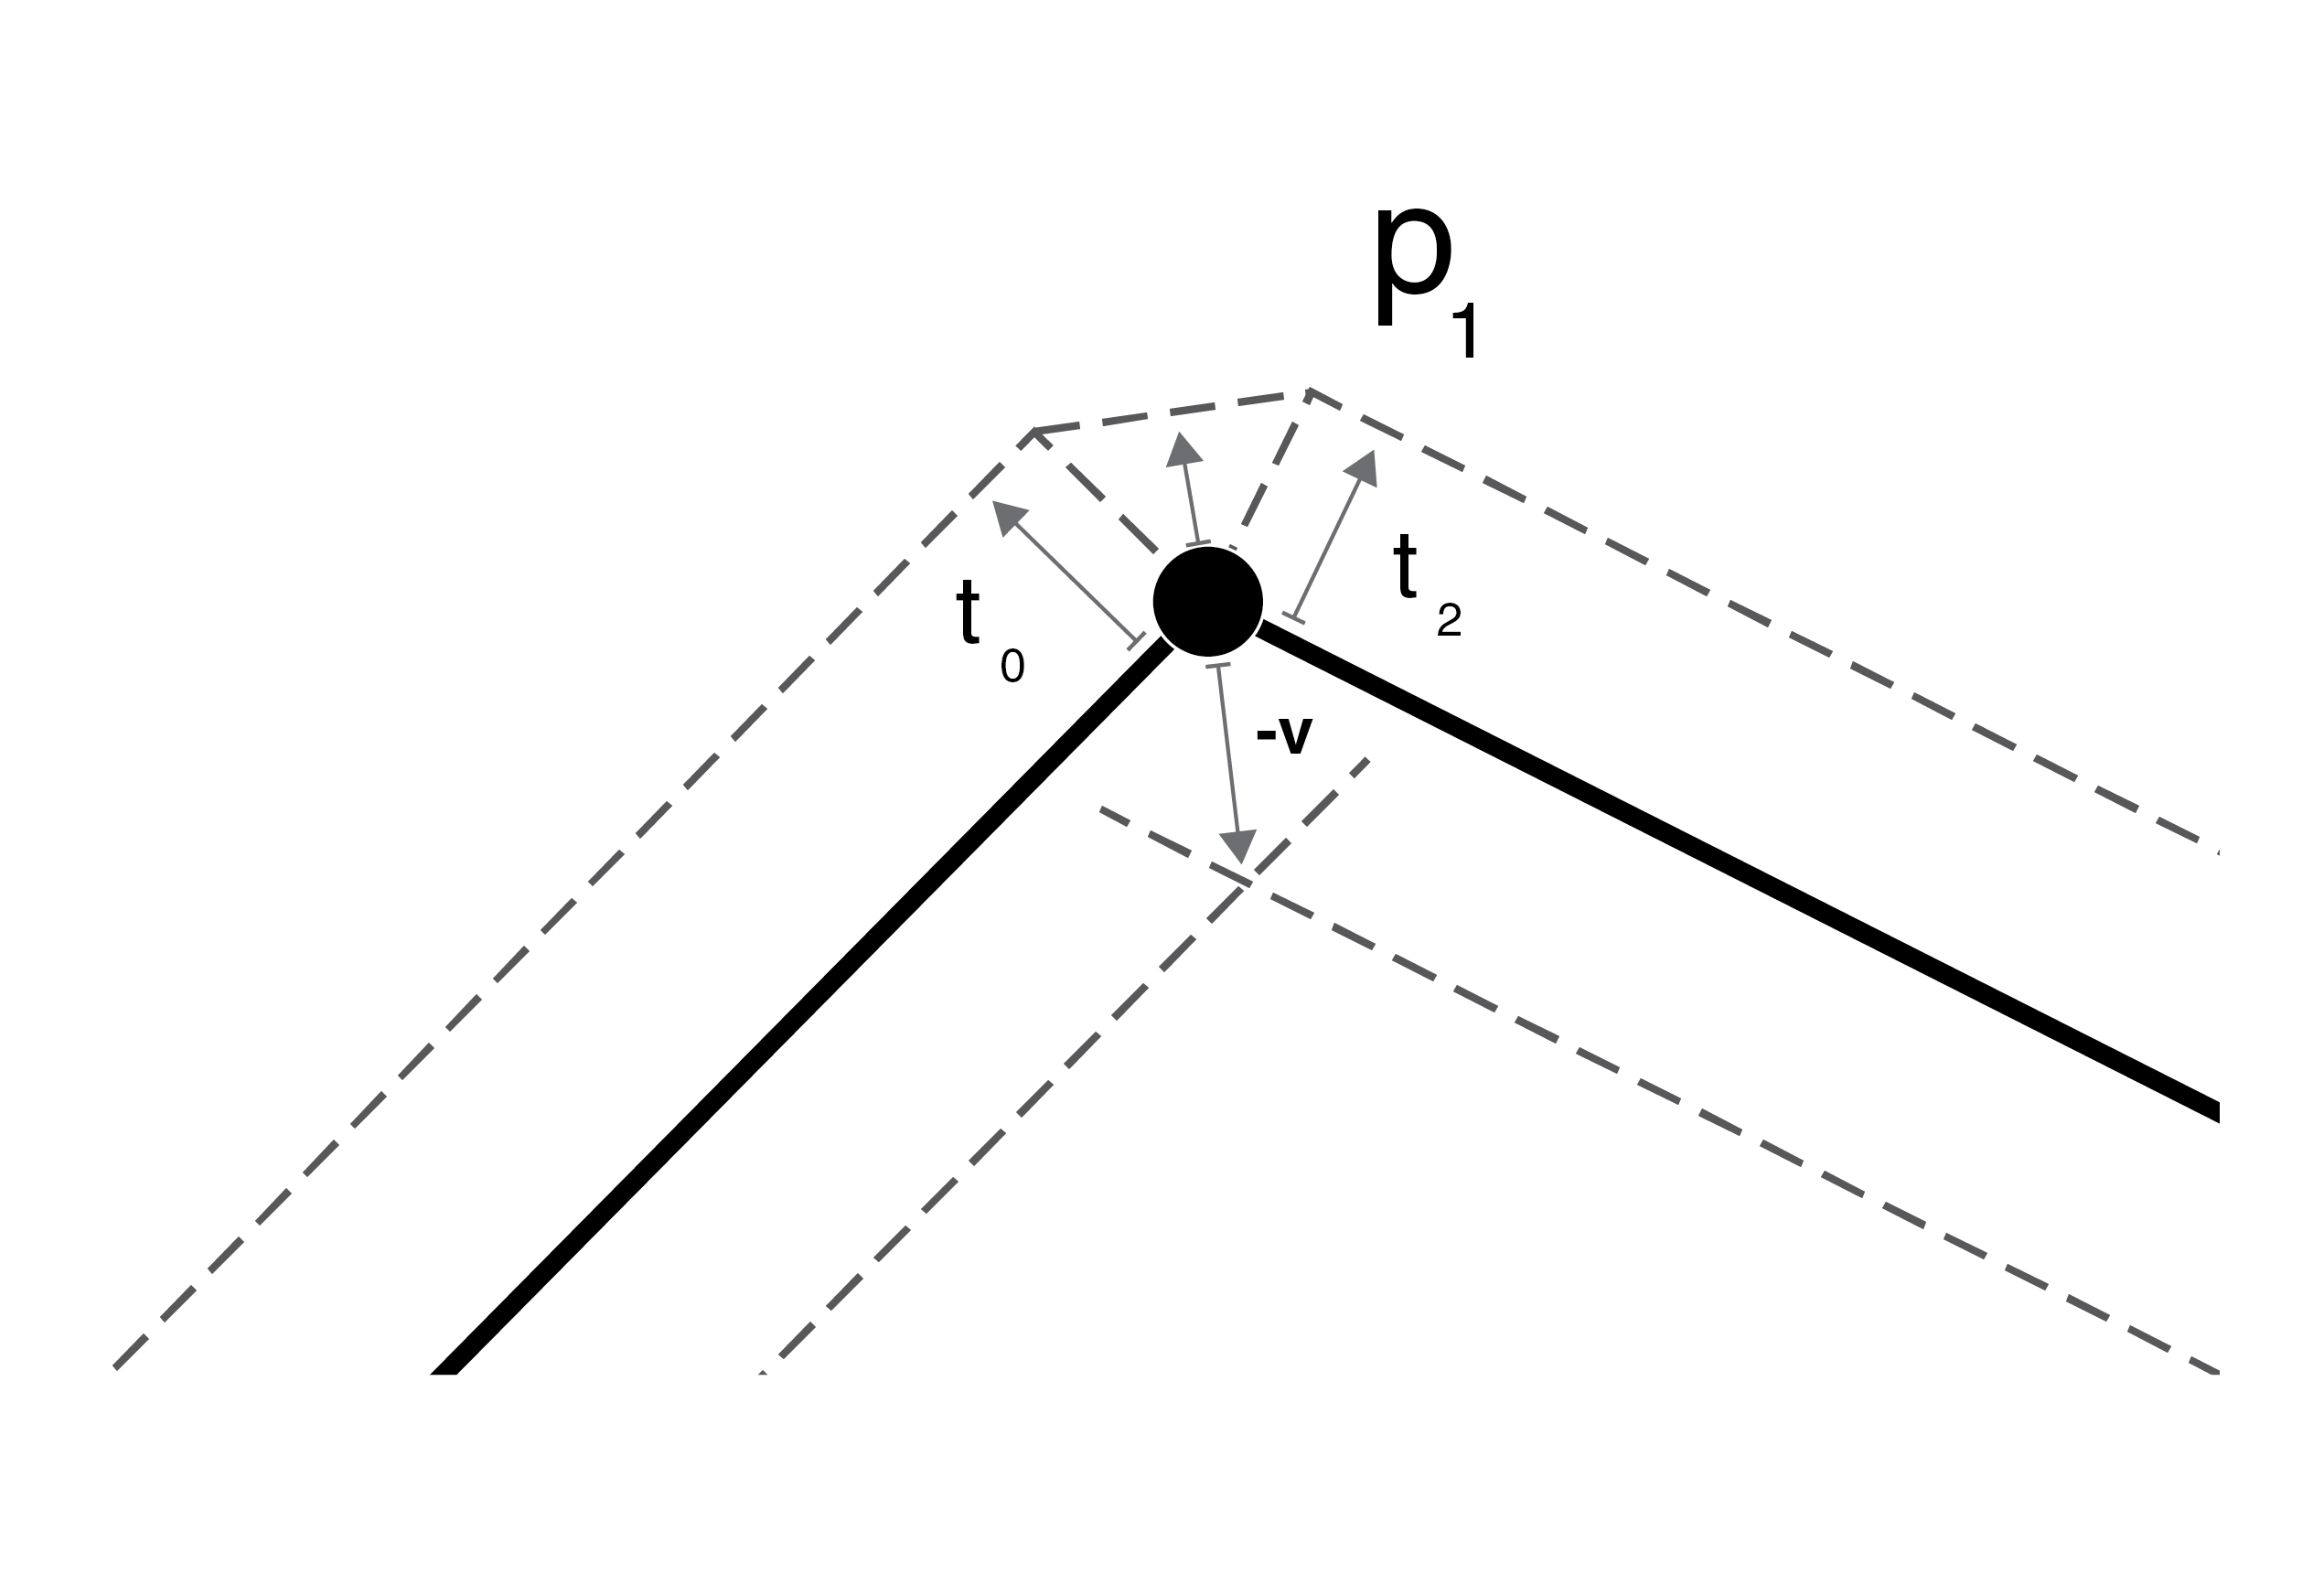
\includegraphics[width=0.7\textwidth]{bevel.png}
\caption[Bevel Join Diagram]{Diagram of a bevel join with parameter labels}
\label{fig:beveljoin}
\end{figure}



\begin{figure}
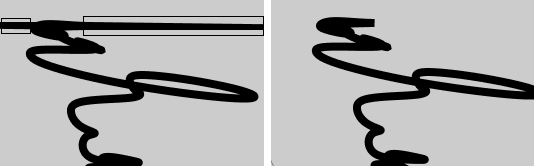
\includegraphics[width=\textwidth]{joinartifact2.png}
\caption[Handling Miter artifacts]{Left: An example of a miter join artifact from a sharp curve. The boxed regions show the artifact. Right: The artifact is detected by calculating the length of the miter join. If detected, the join is replaced with a bevel join.}
\end{figure}

Miter joins have the particular issue that artifacts can arise from exceptionally sharp points in the line segments.
We can detect these cases by checking to see if $v$ is larger than a certain length.
If so, we use a bevel join instead.
The bevel join is formed by simply creating a triangle between $p_1$, $p_1 + \vec{t_0}$, and $p_1 + \vec{t_2}$ (Figure~\ref{fig:beveljoin}).

\subsection{Curved Lines with Variable Width}
Up until this point, we have worked under the assumption that the width of the curved line is constant.
However, we would like to support the ability to draw curved lines that have variable width.
To achieve this, each point on the curve is given an independent width variable, $w_i$.
Assuming we work with three points, we must also define new vectors $t_0$, $t_{01}$, $t_{12}$, and $t_2$ based on the normals of the line segments and the widths at each of the curve points.
Same adjustments need to be made in the join calculations to account for this. 
The miter calculation needs to take the new $t$ vectors into account, turning $(p_0 + \vec{t_0}, p_1 + \vec{t_0})$ and $(p_2 + \vec{t_2}, p_1 + \vec{t_2})$ into $(p_0 + \vec{t_0}, p_1 + \vec{t_{01}})$ and $(p_2 + \vec{t_2}, p_1 + \vec{t_{12}})$.
For a round join, a linear interpolation is used to calculate the radius at the points of triangularization.
The bevel join has no changes in calculation.
The final triangulations also change accordingly.

\section{Implementation}

\begin{figure}
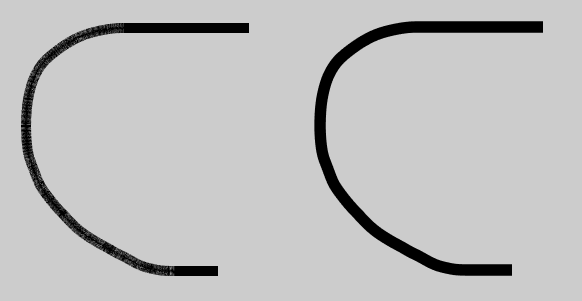
\includegraphics{linerendering}
\caption{Left: A curve using default GL\_LINES. Right: Implemented system}
\end{figure}

Creating this representation geometry can rapidly increase the size of the data, especially as more and more lines are drawn. 
A simple polygonalization for a robust miter and bevel join implementation can create as many as six polygons for each pair of points on the curve.
This does not take into account round joins, as smooth circle approximations require an even larger number of small polygons.
By combining this characteristic with spline subdivision, we run the risk of running into bandwith problems when transferring polygon data between the GPU and the CPU for very large or complex strokes.
To solve for this, we implement these algorithms in a geometry shader using a line adjacency data structure input (Figure~\ref{fig:lineadjacency}).
In order to reduce the number of branch operations, we polygonalize each line segment in halves, taking care of the join calculation for each side separately.
An example of a polygonalized line segment can be seen in Figure~\ref{fig:linepoly}.

\begin{figure}
	\begin{center}
		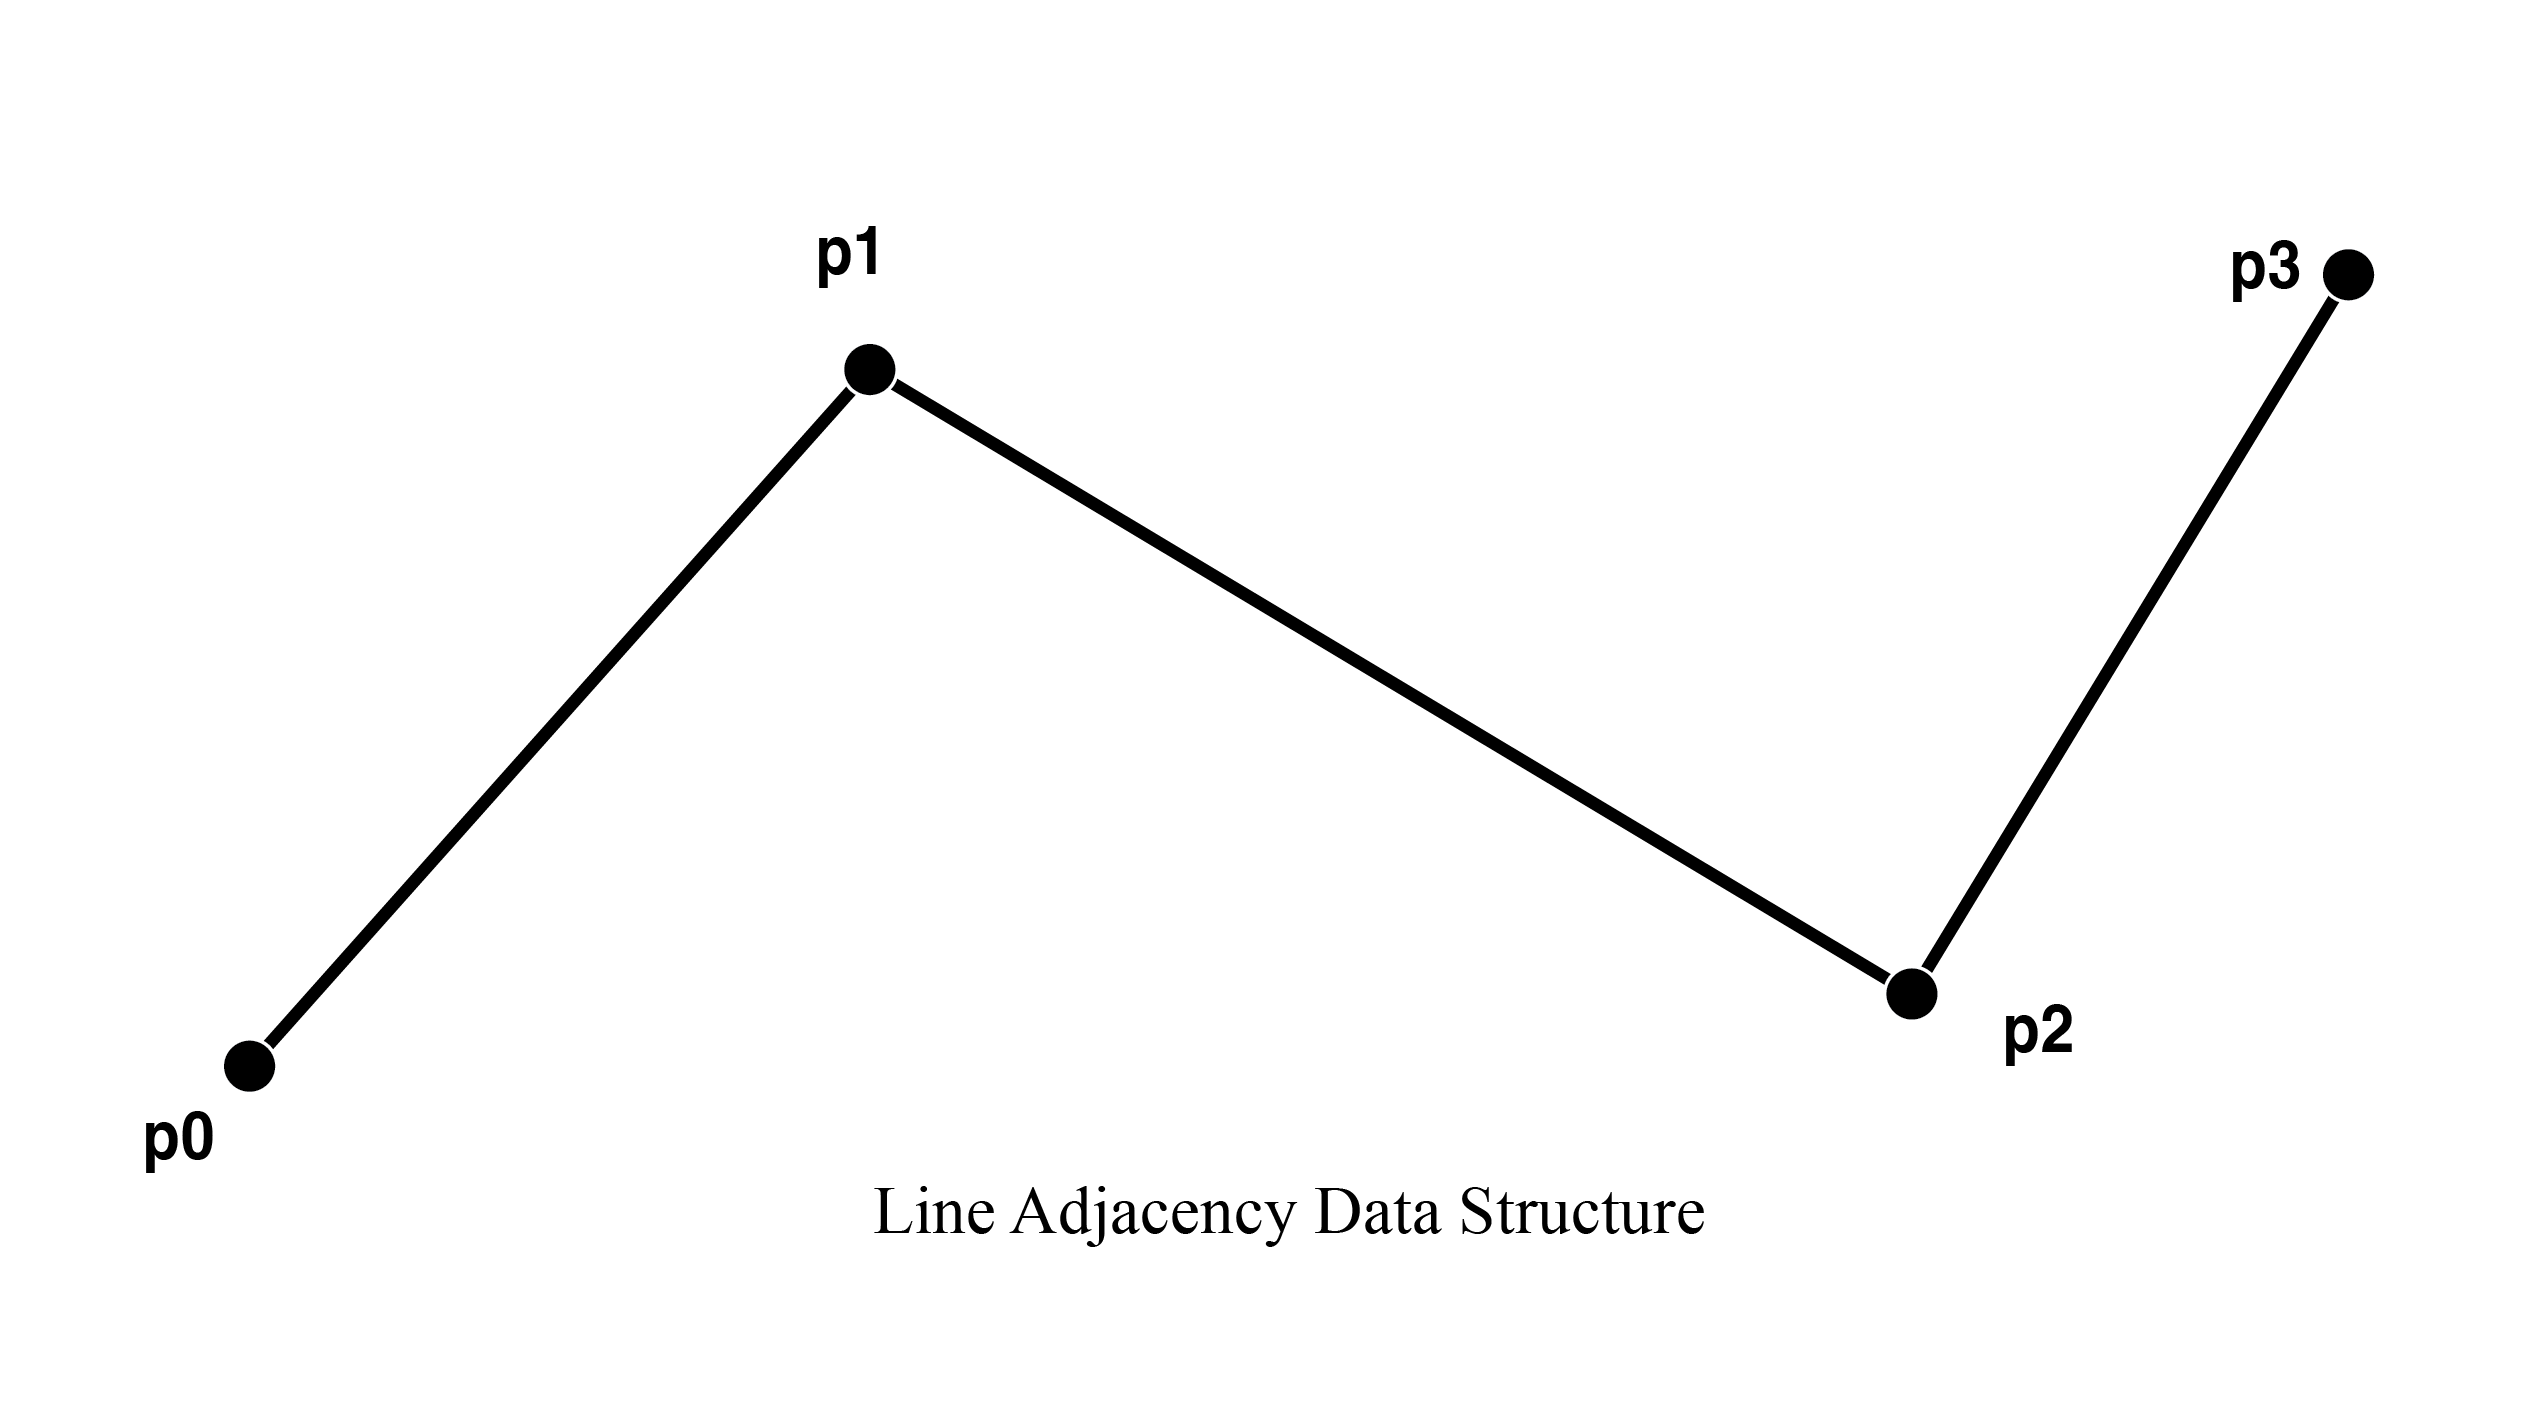
\includegraphics[width=\textwidth]{lineadjacency.png}
	\end{center}
	\caption[Line Adjacency data structure]{Our geometry shader makes use of the line adjacency data structure to generate the curve geometry. Each instance of the geometry shader uses a set of four ordered points ($p_0$, $p_1$, $p_2$, $p_3$) to generate geometry for the line segment ($p_1$, $p_2$)}
	\label{fig:lineadjacency}
\end{figure}
\begin{figure}

	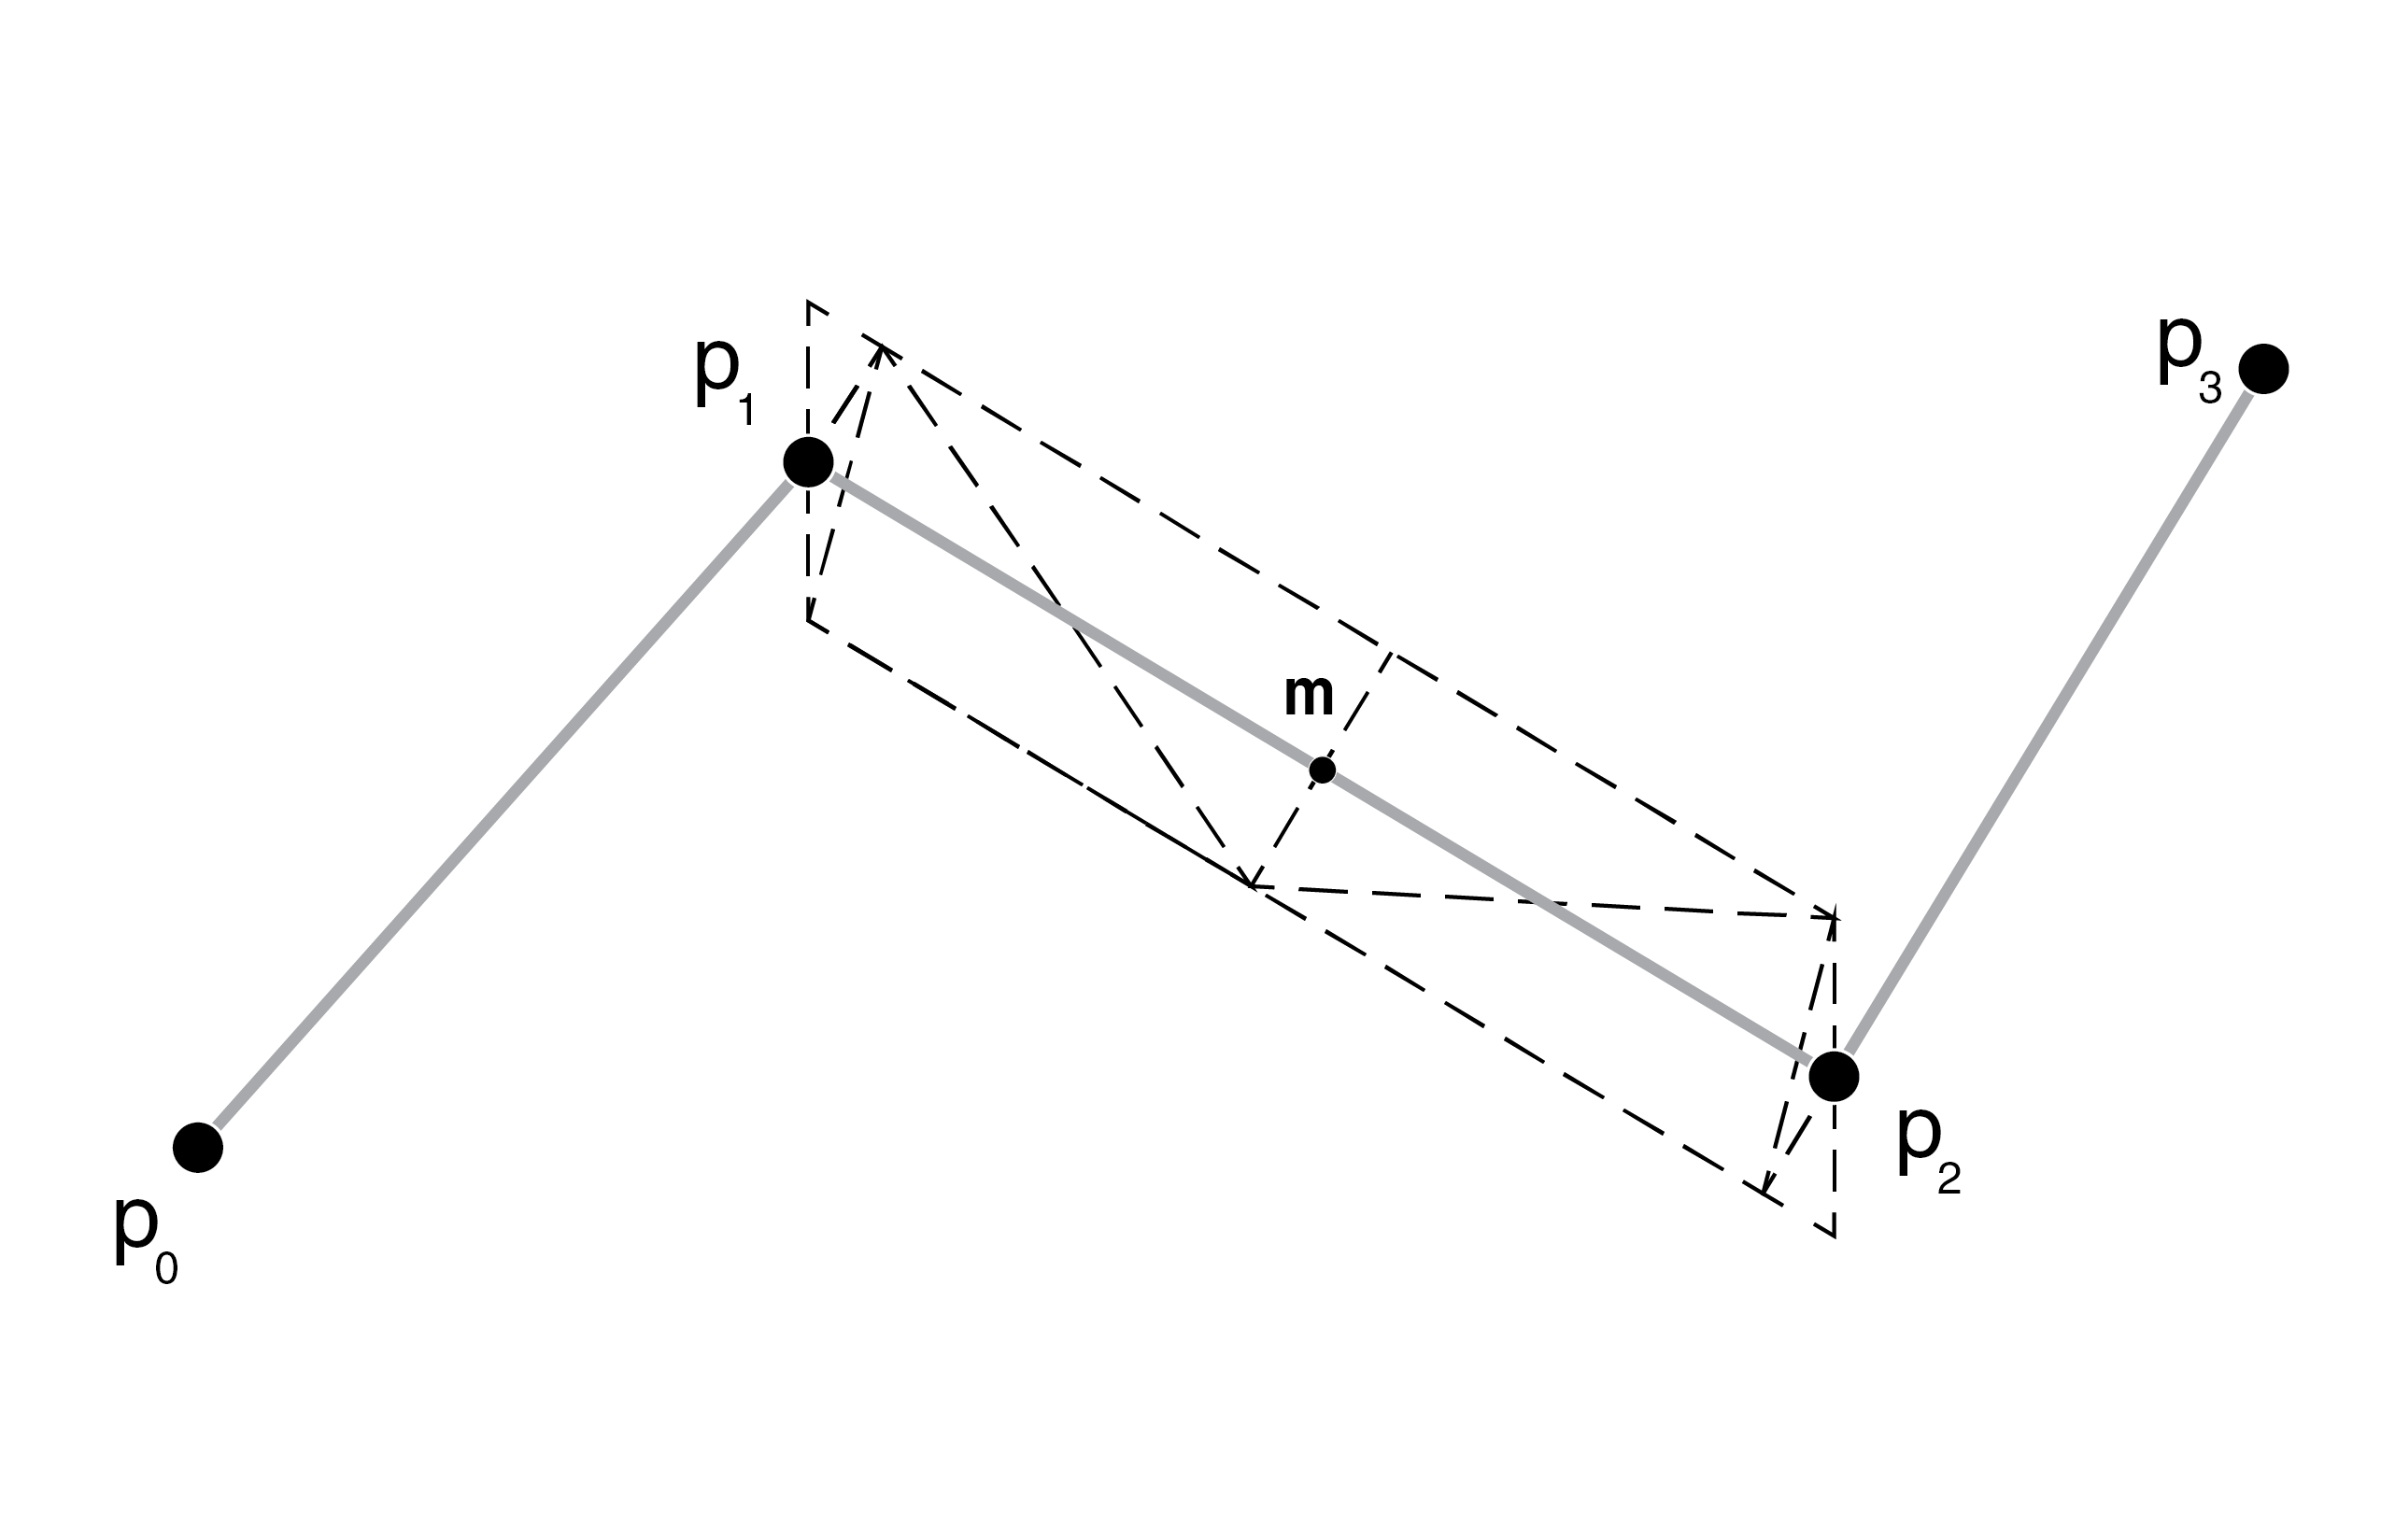
\includegraphics[width=\textwidth]{linepolyex.png}
	\caption[Example polygonization of a line with miter joins.] {Since geometry is only created for the line segment ($p_1$, $p_2$), we need to polygonalize our geometry in such a way that the entire line is rendered correctly. We do this by polygonalizing half of the join for each line segment.}
	\label{fig:linepoly}
\end{figure}



Using the routines described above, the system can now display polygonalized, three dimensional lines efficiently.
However, we still need to decide in what plane we create the line geometry.
The approach CATIA~\autocite{catia} takes is creating the line geometry on the screen and projecting it onto scene objects. 
With this approach, lines only exist on the plane they are drawn on. 
As a result, it is possible to turn the camera such that the camera is perpendicular to the drawing plane and not see already drawn strokes.
This approach is only suitable for applications where a base geometry is already supplied, and therefore not suitable for early stage design applications. 
Other shortcomings include the requirement of a large number of ray cast operations for each line created.
Each segment of the polygonalized curve requires a ray cast operation per polygon vertex. 
This puts too much work on the CPU for a real time application.

We would like to allow for lines to be viewed from any direction, while still retaining their original line width and quality.
The approach our application takes is to perform all of the calculations from creating line geometry in the distorted image space, the space defined after the model is transformed by the model, view, and projection matrices.
By working in the distorted image space, we can guarantee the geometry is always expanded in a plane parallel to the view plane.
The reason we work in the distorted image space as opposed to view space, the space before the projection matrix is applied, is we would like our lines to have a consistent width regardless of depth.
This is because if we were to combine depth altering width with variable sketching width the sense of depth quickly becomes confusing.
This choice is a design decision made after speaking to various architects about the importance of being able to draw lines with different widths.

\begin{algorithm}
\caption{Line Rendering Algorithm}
\begin{algorithmic}
\For{Line Adjacency data set \{$p_0$, $\cdots$, $p_3$\}}
\State{Convert world space line points \{$p_0$, $\cdots$, $p_3$\} to the distorted image space 
\State points \{$p_{0s}$, $\cdots$, $p_{3s}$\}}.
\State Compute normals for each of the line segments $(p_{ns},p_{(n+1)s})$. Normals are 
\State enforced to be pointing towards the outer arcs of segment pairs.
\State Compute join parameters using image space variables and a defined line 
\State width.
\State Triangulate for the line segment ($p_1$, $p_2$)
\EndFor
\end{algorithmic}
\end{algorithm}

\begin{figure}
\begin{center}
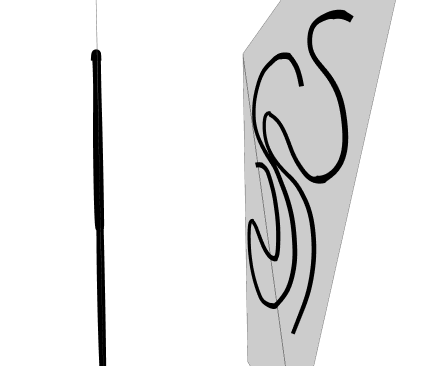
\includegraphics[width=0.5\textwidth]{rotation.png}
\caption{Even when rotating the drawing plane such that it is no longer visible, our lines remain visible.}
\end{center}
\end{figure}

\section{Color}

\label{sec:3dcolor}
One might have noticed that all of the sketches shown so far have been done in black ink.
Unfortunately, colored ink is not possible in our current system.

Before talking about the 3D case, we should talk about the representation of color in a vector 2D graphics environment.
For example, assume we have a vector image with two circles of different color overlapping each other.
The visibility of the circles is determined by their draw order.
However, if we were to look at this in anther way, what is happening is the circles are given a hidden depth value outside the 2D image plane that is related to the draw order.
This "depth" allows for an easy way to determine visibility of colors in vector environments. (Figure~\ref{fig:vecoverlap})

\begin{figure}
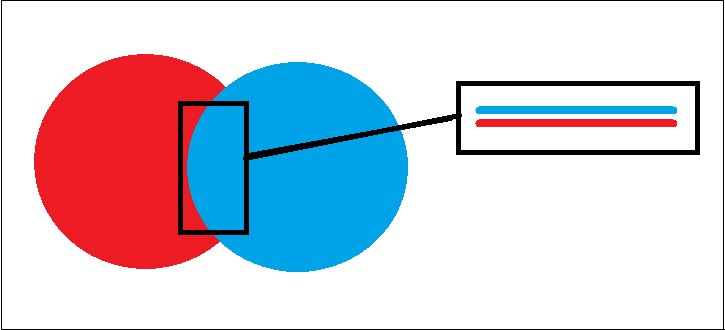
\includegraphics[width=0.9\linewidth]{vectoroverlap}
\caption[Overlapping Colored Objects in 2D Vector Graphics]{When objects of two different colors overlap in a vector graphics environment, a hidden depth value is used to determine visibility.}
\label{fig:vecoverlap}
\end{figure}

However, in a 3D sketching environment, this "depth" cannot be used to accomplish the same result, as in a 3D environment, depth is already defined.
In our system, when two strokes intersect on the same surface, the 3D coordinates are identical.
In graphics hardware, the z-coordinate of a point in NDC space determines visibility.
When two transformed polygons have the same xyz coordinates, we encounter an issue known as Z-fighting, where the two pieces of geometry "fight" over which one is visible.
This manifests as flickering and bizarre appearing geometry at intersections.
When all of the strokes are the same color, the artifacts exist but are not visible.
Because of this, we cannot sketch in multiple colors without including Z-fighting artifacts.

\section{Summary}

In this chapter we have described a method for creating geometry from a sketched line defined by its input sample points.
We have also described how we create it's representation as a 2-D geometry such that the representation is visible from any 3-D direction.
By creating our geometry exclusively on the GPU, we minimize the bandwidth needed to transfer data from the CPU to the GPU, allowing extremely detailed curves using our subdivided spline calculations.